%\pagenumbering{arabic}%start arabic pagination from 1 

\chapter{Platforma Vert.x}

Dnešním trendem internetu jsou aplikace, kde klienti komunikují v reálném čase, proto se také často označují jako kolaborativní aplikace. Tyto aplikace s sebou přinesly drastickou změnu potřeb programátorů na jednotlivé nástroje. Často programátor zjistí, zda-li se mu výběr podařil až v pokročilé fázi vývoje, kdy už nevede cesta zpět. Objevilo se několik nástrojů, které přinesli revoluci na poli webových aplikací. Mezi ně patří například Node.js, Akka nebo Ruby Event Machine. 
Tyto nástroje si vydobyly své místo nejen pro možnost škálování na desítky tisíc klientů, což není v dnešní době nic neobvyklého. 

Vert.x je projekt vycházející z Node.js, který podnítil závod o pokoření C10K\footnote{C10K problém řeší otázku: „Jak je možné obsloužit deset tisíc klientů za pomocí jednoho serveru, a to s co možná nejnižším zatížením serveru} problému. Obě platformy poskytují asynchronní API, které si je co do zaměření velice podobné. Node.js, jak již název napovídá je napsán v jazyce JavaScript, zatímco Vert.x je implementován v Javě. Vert.x ale není pouhá reimplementace Node.js do jazyka Java. Platforma má svou vlastní unikátní filozofii a terminologii, která je diametrálně odlišná od Node.js.

\section{Historie}

Začátek vývoje projektu Vert.x je datován do roku 2011. Tedy rok poté co spatřil světlo světa framework Node.js. Vert.x si za pouhý rok vydobyl své místo u komunity, která si jej velmi oblíbila. 

Hlavním autorem platformy je Tim Fox, který v době začátku vývoje platformy pracoval ve společnosti VMWare. Tato společnost si vzápětí nárokovala všechny zásluhy Tima Foxe na Vert.x platformu. Právníci společnosti vydaly výzvu, ve které požadovali mimo jiné doménu, veškerý zdrojový kód a účet Tima Foxe na Githubu. Z toho důvodu Tim Fox odešel od společnosti v roce 2012. V témže roce projevila o platformu zájem firma RedHat, která nabídla Timovi nejen pracovní místo, ale i absolutně volnou ruku ve vývoji a vedení projektu\citep{whoControlVertx}. 

Po několika debatách jak s představiteli společnosti RedHat tak i komunitou, došel Tim Fox k názoru, že nejlepší pro budoucnost a zdravý rozvoj platformy bude přesunutí celé platformy pod nadaci Eclipse Foundation, k čemuž došlo na konci roku 2013. V dnešní době se platforma těší velkému vývoji, který čítá desítky  pravidelných přispěvatelů mezi něž patří mimo Tima například Norman Maurer, který se řadí mezi přední inženýry vyvíjející framework Netty.io\footnote{framework pro práci se vstupy a výstupy} a zodpovídá za integraci Netty.io frameworku do platformy Vert.x\cite{vertxNodejs}.
Letos Vert.x vyhrál prestižní cenu "Most Innovative Java Technology" v soutěži JAX Innovation awards\citep{JAX}.

\section{Architektura}

\begin{figure}[h]
\begin{centering}
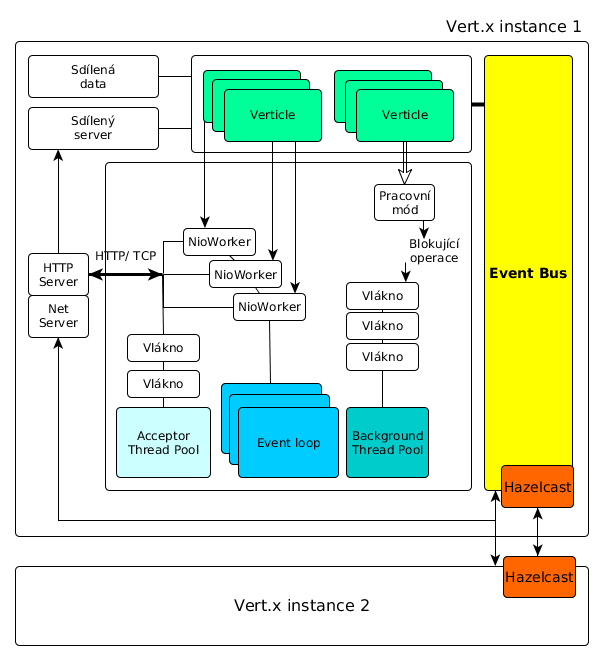
\includegraphics[scale=0.55]{obrazky/architecture_vertx}
\par\end{centering}
\caption{Architektura Vert.x převzato a upraveno z \cite{vertxArchitectureDiagram} \label{fig:vertxArchitectureDiagram}}
\end{figure}

Na obrázku \ref{fig:vertxArchitectureDiagram} jsou znázorněny dvě nezávislé Vert.x instance, které spolu komunikují pomocí zpráv. V levé části je blíže zobrazena jedna Vert.x instance, která bude blíže rozebrána v následujících kapitolách.

\subsection{Jádro}

Velikost samotného jádra aplikace nepřekračuje 10Mb kódu v jazyce Java. V současné verzi je jádro platformy koherentní, dobře čitelné a poskytuje malé, ale za to stabilní API. Jak je popsáno v kapitole \ref{sub:API}, Vert.x se nesnaží umět vše, ale specializuje se na určitou oblast. Díky těmto faktům je snadno rozšiřitelný a integrovatelný. Lze jej rozšířit o novou funkčnost pomocí balíčků, které lze naleznout v oficiálním repozitáři. Pravděpodobnou inspirací byl již zmíněný Node.js, který se svým výkonem vydobyl své místo. Samotnou inspirací byly podle Tima Foxe Node.js a ERLang\cite{vertxNodejs}.

\noindent Zásadní technologie, které integruje Vert.x.
\begin{description}
\item[Netty.io] framework pro práci se vstupy a výstupy
\item[Hazelcast] In-memory data grid\cite{inMemoryDataGrid}
\end{description}

Netty.io samotný, lze použít pro vývoj webových aplikací stejně dobře jako kterýkoliv jiný nástroj. Jeho specializací však je práce se vstupy a výstupy tzv. IO. V této oblasti poskytuje nízkoúrovňové API, nad kterým Vert.x přidává vyšší míru abstrakce. Druhou technologií, která je pro Vert.x klíčová je popsána v samostatné kapitole \ref{sub:hazelcast}.

\subsection{Asynchronní model}

Událostmi řízené programování je podle Tomáše Pitnera\cite{javaProgramovani} základním principem \\tvorby aplikací s GUI. Netýká se však pouze GUI, je to obecnější pojem označující typ asynchronního programování, kdy je tok programu řízen událostmi, na které navěšuje tzv. event handlery\footnote{obslužná rutina události}. Typy událostí na které lze reagovat:

\begin{itemize}
\item Událost přes GUI
\item Chyba
\item Zatížení
\end{itemize}

Události nastávají obvykle určitou uživatelskou akcí (klik či pohyb myši, stisk tlačítka).
Událostmi řízené aplikace musí být většinou programovány jako vícevláknové (i když spouštění vláken obvykle explicitně programovat nemusíme).
Asynchronní někdy také paralelní model je přímo závislý na způsobu implementace samotným programovacím jazykem. Základním pojmem je zde proces, který je vnímán jako jedna instance programu, který je plánován pro nezávislé vykonávání. Naproti tomu Vlákno\footnote{Označuje v informatice odlehčený proces, pomocí něhož se snižuje režie operačního systému při změně kontextu, které je nutné pro zajištění multitaskingu} je posloupnost po sobě jdoucích událostí. V dřívější době nebylo potřeba rozlišovat proces a vlákno, protože proces se dále v aplikaci nedělil. Vytvoření vlákna je poměrně drahá a pomalá operace. Což se často obchází vytvořením zásoby uspaných vláken dopředu s nějakým managementem, který vlákna přidává a ubírá dle potřeby. Základním principem Vert.x a jemu podobných frameworků je hlavní vlákno, obvykle pro každý procesor jedno. Takové vlákno si samo řídí vytváření a přidělování vláken.

Tento model bývá často kritizován, že nutí programátory psát špatně udržovatelný kód, především v situacích, kdy je potřeba koordinovat výsledky mezi více handlery. Pro tyhle situace ovšem vznikla řada nástrojů, které se liší podle použitého jazyka.

%respektive Node.js je tedy jedno hlavní vlákno, které si dle potřeby vytváří vlákna další a řídí tak . V jedné aplikace tedy může běžet několik vláken. Vlákno je zde bráno jako základní plánovací jednotka pro běh na procesoru. 
%Existují dva druhy asynchronního modelu (multitaskingu):
%multiprocesorový: o běh, tvorbu a režii vláken se stará operační systém
%multivláknový: o běh, tvorbu a režii vláken se stará aplikace a předává je operačnímu systému
%Podle Lažanského\cite{vlaknaCvut} je sdílení paměti důsledkem nižší režie při přepínání (přepnutí %vláken je výrazně rychlejší), obdobně i vytváření a rušení vlákna a samozřejmě i úspora paměti.
Samotné jádro Vert.x je implementováno v jazyce Java a pro Vert.x je tedy důležité, jak moc je dobrá implementace paralélního modelu v tomto jazyce. Neznamená to však, že se celá aplikace musí implementovat výhradně v jazyce Java. Jediný požadavek pro běh Vert.x instancí je přítomnost Java development Kitu ve verzi 1.7 a novější. Tato verze přinesla nespočet vylepšení, pro jejichž výpis zde není místo. Došlo také na reimplementaci či úpravy v několika zásadních třídách z balíčku java.util.concurrent, což je třída zabývající se prací s multitaskingem a konkurencí.
\begin{description}
\item[ExecutorService]{z balíčku java.util.concurrent}
\item[CyclicBarrier\footnote{Synchronizační bariéra. Využitelná pro konstantní skupinu vláken, které mají přistupovat ke stejné proměnné. Třída zajištuje, že na sebe vlákna musí čekat při přístupu k proměnným. (Cyklická, protože jakmile se uvolní první vlákno jede to samé od znova)}]{z balíčku java.util.concurrent}
\item[CountDownLatch]{z balíčku java.util.concurrent}
\item[File]{z balíčku java.nio}
\item[Vylepšený ClassLoader\footnote{objekt zajištující načítání tříd}]{lepší odolnost vůči deadlockům\footnote{ je odborný výraz pro situaci, kdy úspěšné dokončení první akce je podmíněno předchozím dokončením druhé akce, přičemž druhá akce může být dokončena až po dokončení první akce.}}
\end{description}
\emph{Více o java.concurrent\cite{javaChangelog}}

Ed Gardoh v roce 2011 ve svém jednoduchém testu\cite{serialTest} prověřil práci s paralelizací úkonů. Z jeho testů vyplývá, že Java 1.7 je až o 40\% rychlejší při práci s vlákny nejenom díky nové metodě Fork/Join\cite{forkJoin}.

\subsubsection{Návrhový vzor Reactor}

\begin{figure}[h]
\begin{centering}
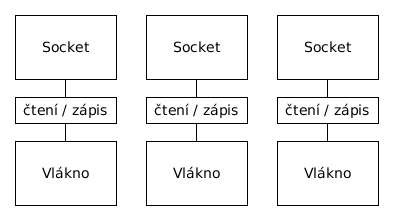
\includegraphics[scale=0.55]{obrazky/blocking_pattern}
\par\end{centering}
\caption{Blokující přístup \emph{převzato a upraveno z \cite{nettyInAction}}\label{fig:blocking_pattern}}
\end{figure}

,,Tradiční" aplikační serverové kontainery rezervují jedno vlákno pro každou I/O operaci. To v praxi znamená jedno vlákno pro jedno spojení. Jak je vidět z obrázku \ref{fig:blocking_pattern}, takové vlákno čeká na odpověď každého řádku volání a prakticky využívá zdroje, které k ničemu nepotřebuje. Což je velice neefektivní přístup. Vert.x využívá návrhového vzoru \emph{Reactor}, který implementuje Netty.io. Vert.x tuto knihovnu využívá jako vestavěný systém. Jeden z hlavních vývojařů Netty.io, Norman Maurer a autor knihy Netty in action\cite{nettyInAction} pracuje na integraci s Vert.x platformou. Z obrázku \ref{fig:vertx_pattern} je patrné, že vzor spočívá v běhu jednoho vlákna, kterému tzv. ,,Selector" podává požadavky.

\begin{figure}[h]
\begin{centering}
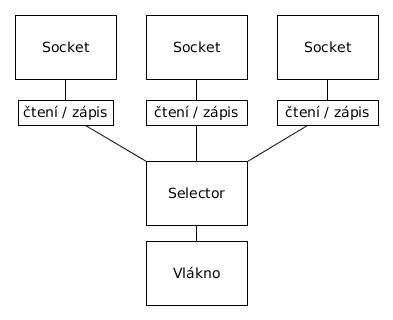
\includegraphics[scale=0.55]{obrazky/vertx_pattern}
\par\end{centering}
\caption{Neblokující přístup pomocí Netty.io \emph{převzato a upraveno z \cite{nettyInAction}}\label{fig:vertx_pattern}}
\end{figure}

\subsubsection{Event loop}

Event loop využívá Netty.io NioWorkery. Každý verticle\footnote{nejmenší jednotka Vert.x více v kapitole Terminologie \ref{sub:verticle}} má vlastního NioWorkera, díky tomu je zaručeno, že každé verticle je jedno vláknové. Základem asynchronního modelu je vlákno, které se stará o všechny události. Když událost dorazí vlákno se postará o to aby byla zavolána ta správná obslužná rutina. Každá Vert.x instance interně obsluhuje malý počet těchto vláken, zpravidla jedno na každé procesorové jádro. Těmto vláknům se ve Vert.x komunitě říká \emph{Event Loop}. V komunitách Nginx nebo Node.js se ovšem setkáme spíše s pojmem \emph{Run Loop}. Přeloženo volně do češtiny ,,událostní smyčka". Obrovská nevýhoda takového přístupu je, že nikdy nesmí dojít k blokování hlavního vlákna. Jakmile k tomu dojde, celá aplikace tzv. zamrzne. Při startu verticlu \ref{sub:verticle} je vybrán jeden event loop, který ho obsluhuje po celý životní cyklus. Event loop je schopný obsloužit tisíce verticlů v ten samý čas. Příklady blokujících volání:
\begin{itemize}
\item{tradiční API (JDBC, externí systémy)}
\item{dlouhotrvající operace (generování apod.)}
\end{itemize}

\subsubsection{Návrhový vzor Multi-reactor}\label{sub:multireactor}

Základ jádra je postaven na tzv.
Multi-reactor pattern\cite{eventLoops}, který vychází z Reactor 
patt-ernu\cite{reactorPattern}. Ten lze charakterizovat několika body:

\begin{itemize}
\item{aplikace je řízena událostmi}
\item{na události se registrují handlery}
\item{vlákno zpracovává události a spouští registrované handlery}
\item{toto vlákno nesmí být blokováno\footnote{pokud dojde k zablokování hlavního vlákna dojde k zablokování celé aplikace např.\emph{Thread.sleep(), a další z java.util.concurrent }}}
\end{itemize}

Multi-reactor pattern\cite{eventLoops} se od Reactor patternu liší pouze tím, že může mít více hlavních vláken. Tím přináší Vert.x možnost pohodlně škálovat instance na více procesorových jader. Jak je vidět z obrázku \vref{fig:instance} Vert.x platforma poskytuje více hlavních vláken, zpravidla však jedno hlavní vlákno na jeden procesor. Toho lze snadno docílit pomocí \emph{Runtime.getRuntime().availableProcessors()}, o kterém se dozvíte více v kapitole \ref{sub:Scaling}. Na obrázku \vref{fig:instance4} lze vidět situaci čtyř hlavních vláken na čtyři procesorová jádra.

\subsubsection{Hybridní model vláken}\label{sub:hybrid}

Platforma Vert.x přišla s inovací v oblasti hlavních vláken a to takovou, že k hlavním \emph{Event loops} přidala další sadu vláken \emph{Background thread pool}, které jsou vyčleněny z hlavní architektury a poskytují samostatnou kapitolu pro škálování aplikace. To lze ostatně vidět na obrázku \vref{fig:vertxArchitectureDiagram}. Díky tomu, lze psát specializované moduly nebo verticle tzv. \emph{workery} pro blokující volání či dlouhotrvající operace aniž by nějak omezovaly běh celé aplikace. Více o \emph{workerech} v kapitole \ref{sub:moduly}.

\subsection{Terminologie}

Vert.x definuje svou vlastní terminologii, která je specifická jen pro tuto platformu. Před dalším výkladem je tak nutné porozumět jednotlivým pojmům, které budou vysvětleny v následujících podkapitolách.

\subsubsection{Verticle}\label{sub:verticle}

Verticle je základní jednotka vývoje a nasazení, lze si ji představit jako kus kódu nebo třídu s hlavní metodou. Verticle je tak nejmenší funkční jednotkou Vert.x. Verticle lze spouštět samostatně přímo z příkazové řádky podobně jako skript. Každý verticle běží ve vlastním vlákně z čehož plynou výhody, ale také nevýhody. Vzhledem k tomu, že každý verticle má svůj vlastní classloader nemůže, tak sdílet statické metody ani hodnoty proměnných s ostatními. Naopak výhodou je, že programátorovi odpadnou starosti s nejrůznější synchronizací vláken či zámky nad proměnnýma. V případě jedno vláknového modelu také odpadají nepříjemné deadlocky. Výzvou je sdílení dat mezi jednotlivými komponentami aplikace, které lze v případě Vert.x sdílet dvěma způsoby:
\begin{itemize}
\item{pomocí Message Queue\cite{mq} dále jen MQ}
\item{SharedData object a SharedSet \emph{vertx.sharedData()}}
\end{itemize}
Objekty v SharedData musí být immutable\footnote{jakmile jednou takovýto objekt vznikne nejde dále měnit jeho proměnné}. V dnešní době je řada MQ frameworků přes které lze vést komunikaci. U platformy Vert.x však není potřeba externí služba, protože má vlastní Event Bus, o kterém pojednává kapitola \ref{sub:eventBus}. Na obrázku \ref{fig:instance} je vidět jeden verticle v kontextu jedné Vert.x instance. Následuje sumarizace vlastností verticlu:
\begin{figure}[h]
\begin{centering}
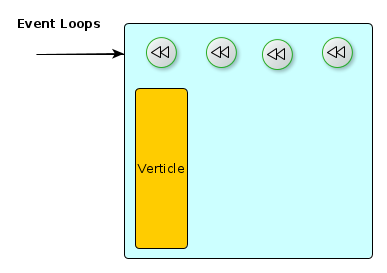
\includegraphics[scale=0.5]{obrazky/instance}
\par\end{centering}
\caption{Vert.x instance \label{fig:instance}}
\end{figure}

\begin{itemize}
\item nejmenší spustitelná jednotka
\item třída / skript
\item vykonává neblokující operace
\item běží vždy v jednom vlákně
\item přímý přístup k API, registrace handlerů, nasazení dalších verticlů
\end{itemize}

\subsubsection{Worker verticle}

V standardním verticlu by nemělo nikdy dojít k blokování hlavního vlákna. V dnešní době se bez klasického synchronního volání pravděpodobně neobejdeme, protože většina knihoven a modulů je napsána jako blokující kód. Z toho důvodu je v platformě Vert.x možnost označit verticle jako workera, respektive pustit jej jako worker verticle metodou \emph{deployWorkerVerticle} namísto \emph{deployVerticle}. Tím dojde k vyčlenění verticle z asociace na hlavní vlákna a takovému vláknu bude přiděleno vlákno z Background thread poolu. Uvnitř takového verticle lze vykonávat blokující volání bez blokování celé aplikace. To v praxi rozšířilo možnosti uplatnění celé platformy. Bohužel tímto ztrácíme efektivní možnost škálování pro velký počet konkurenčních vláken. Je tedy vhodné situovat náročné výpočty na speciálně vyčleně servery. Velikost background thread poolu ve výchozím nastavení čítá 20 vláken. Jak tento počet změnit je popsáno v kapitole \ref{sub:performenceScale}.

\subsubsection{Vert.x instance}

\begin{figure}[h]
\begin{centering}
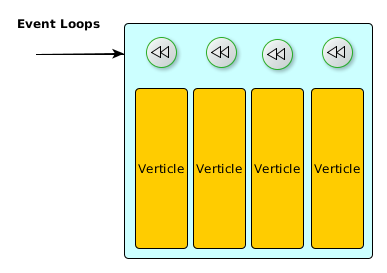
\includegraphics[scale=0.5]{obrazky/instance4}
\par\end{centering}
\caption{Příklad vertikálního škálování \emph{vertx run HelloWord -instances 4} \label{fig:instance4}}
\end{figure}

Každý verticle běží uvnitř Vert.x instance \vref{fig:instance} a každá instance běží ve vlastní JVM\footnote{Java Virtual Machine} instanci. V jedné Vert.x instanci může najednou běžet nespočet verticlů. Z obrázku \ref{fig:scaling_example} je patrné, že se jedná o vertikální druh škálování. Kdy na jednom serveru běží více Vert.x instancí. Počet instancí je zpravidla roven počtu procesorů, větší počet má negativní dopady na rychlost aplikace. Nastane situace, kdy se jednotlivá vlákna přetahují o procesorový čas.

\subsubsection{Moduly}\label{sub:moduly}

Moduly poskytují možnost zapouzdření a znovupoužitelnost funkcionality. V praxi se mohou moduly skládat z více modulů či verticlů ve více programovacích jazycích. Moduly mohou být uloženy v centrálním repozitáři\footnote{http://modulereg.vertx.io/} nebo může být využit jakýkoliv jiný repozitář. Repozitáře, ve kterých hledá Vert.x při startu instance dostupné moduly lze definovat v souboru \emph{conf/repos.txt} nacházející se v kořenové složce Vert.x. Každý modul musí mít svůj deskriptor ve formátu JSON\footnote{je odlehčený formát pro výměnu dat}. Ukázka deskriptoru je v kapitole \ref{sec:praktickyModuly}.

Výhody plynoucí z použití modulů:
\begin{itemize}
\item{classpath\footnote{říká JVM, kde má hledat třídy a balíčky} je zapouzdřený a díky tomu lze moduly pouštět mnohem snáze}
\item{všechny závislosti jsou zapouzdřeny v jediném souboru ve formátu ZIP nebo JAR\footnote{java formát založený na formátu ZIP}}
\item{moduly mohou být umístěny v repozitářích}
\item{Vert.x dokáže automaticky stahovat moduly, pokud je nenalezne v lokální instalaci}
\end{itemize}

Typy modulů lze rozdělit do dvou základních skupin, které lze dál rozdělit podle typu určení modulu na:

\begin{description}
\item[spustitelné]{mají definovaný hlavní verticle v deskriptoru, takové moduly je možné spustit jako samostatné jednotky pomocí parametru \emph{runmod} nebo programově \emph{deployModule} }
\item[nespustitelné]{modul nemá specifikovaný hlavní verticle a lze jej použít v jiném modulu definováním parametru \emph{includes} uvnitř deskriptoru modulu}
\end{description}

Pro vyčlenění modulu z asociace na event loop stačí přidat parametr \emph{worker: true} do deskriptoru modulu.

\subsection{Event Bus}\label{sub:eventBus}

\begin{figure}[h]
\begin{centering}
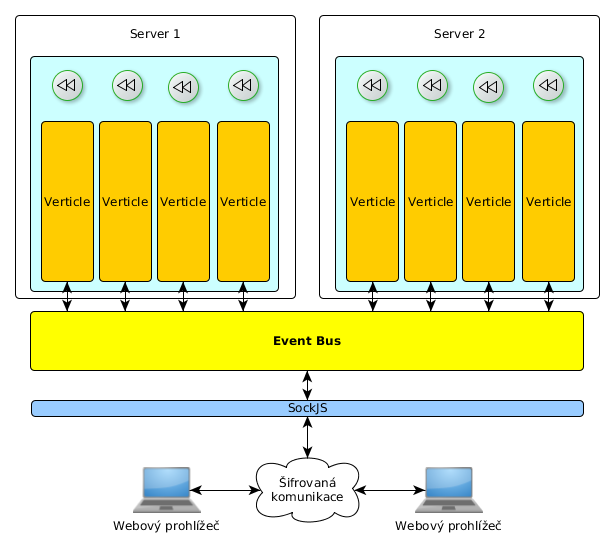
\includegraphics[scale=0.5]{obrazky/2instance4_eventbus}
\par\end{centering}
\caption{Event Bus distribuovaný mezi dva servery}
\label{fig:2instance4_eventbus}
\end{figure}

Nervový systém celého Vert.x, jehož název lze volně přeložit jako sběrnice událostí. Cílem EventBusu je zprostředkování komunikace mezi jednotlivými komponentami a vlákny aplikace. Podobně jako při použití externí MQ. Díky faktu, že komponenta Event Bus je implementována přímo v jádru platformy, odpadá nutnost používat další knihovny pro práci s MQ a v neposlední řadě také režijní náklady či výpočetní výkon. Jak je vidět na obrázku \ref{fig:2instance4_eventbus}, komponenta Event Bus je distribuovaná přes všechny instance v clusteru. Samozřejmostí je možnost přemostění této komunikace do webového prohlížeče, což je detailněji popsáno v kapitole \ref{sec:realTimeCommunication}. Event bus nepřináší v porovnání s profesionální MQ systémy takové možnosti, jako například transakční zpracování, ale již existuje modul pro přemostění komunikace například do RabbitMQ\footnote{MQ napsaná v ERlangu}. S vývojáři RabbitMQ je Tim Fox v úzkém kontaktu\cite{vertxNodejs}. Základní typy komunikace:
\begin{itemize}
\item{Point to Point}
\item{Publish/Subscribe}
\end{itemize}

typy zpráv:
\begin{itemize}
\item{String}
\item{primitivní typy (int, long, short, float double, ..)}
\item{org.vertx.java.core.json.JsonObject}
\item{org.vertx.java.core.buffer.Buffer}
\end{itemize}

Toto je výčet pouze základních typů zpráv, které Vert.x podporuje v jádře. Není ale vůbec problém výčet stávájících typů rozšířit implementací vlastního modulu. Například modul \emph{bson.vertx.eventbus}\footnote{https://github.com/pmlopes/mod-bson-io} rozšíří EventBus o možnost používat mnohem komplexnější typy zpráv:

\begin{itemize}
\item{java.util.UUID}	
\item{java.util.List}
\item{java.util.Map}
\item{java.util.Date}
\item{java.util.regex.Pattern}
\item{java.sql.Timestamp}
\end{itemize}

Mezi doporučené se ovšem řadí JSON, protože je jednoduše serializovatelný mezi jednotlivými programovacími jazyky.

\subsubsection{Hazelcast}\label{sub:hazelcast}

Jednou z nejdůležitějších architektonických součástí Vert.x je knihovna Hazelcast, kterou tvoří jenom neuvěřitelných 3,1MB kódu v jazyce Java. V platformě Vert.x zaujímá důležité postavení jako In-memory data grid, jehož vlastnosti \cite{inMemoryDataGrid} lze podle Ki Sun Song sumarizovat:
\begin{itemize}
\item{Data jsou distribuovaná a uložená na více serverech ve více geografických lokacích}
\item{Datový model je většinou objektově orientovaný a ne-relační}
\item{Každý server pracuje v aktivním režimu}
\item{Dle potřeby lze přidávat a odebírat servery}
\end{itemize}

Hazelcast je tedy typ distribuovaného úložiště, které běží jako vestavěný systém, lze díky němu distribuovat celou aplikaci a zasílat zprávy mezi jednotlivými komponentami. Vert.x API využívá Hazelcast API a odstiňuje tak programátora od poměrně nízko úrovňové API Hazelcastu. Když je Vert.x spuštěn, Hazelcast je spuštěn v módu vestavěného systému. Jako nejčastější příklad užití samotného Hazelcastu bývá uváděno ukládání uživatelské session\cite{session}. Hazelcast tedy usnadní práci v situaci, kdy budeme potřebovat uložit uživatelskou session, například pro eshop. Mohli bychom využít externí RDBMS tedy databázový server, který by obstarával komunikaci s klienty a udržoval integritu dat, díky kterému by jsme dosáhli stejného výsledku. S využitím knihovny Hazelcast ovšem odpadá nezbytná režie a monitoring, nemluvě o serverových prostředcích.
Knihovnu Hazelcast lze využít v několika rolích:
\begin{itemize}
\item{NoSQL databáze v paměti}
\item{Cache\footnote{specializovaný typ paměti pro krátkodobé ukládání}}
\item{Data grid}
\item{Zasílání zpráv}
\item{Aplikační škálování}
\item{Clustrování aplikací}
\end{itemize}

\section{API}\label{sub:API}

Vert.x poskytuje malou sadu metod, kterou lze volat na přímo z jednotlivých verticlů.
Funkcionalitu platformy lze jednoduše rozšířit pomocí modulů, které po zveřejnění do centrálního repozitáře může využívat kdokoliv a pomáhá tak znovu použitelnosti kódu. Samotné jádro Vert.x je tak velice malé a kompaktní. Vert.x API je rozděleno na \emph{Základní API} a \emph{Kontainer API}.

\subsection{Základní API}\label{sub:coreAPI}

V porovnání s většinou nástrojů se může na první pohled zdát, že je Vert.x API strohé. Při hlubším zkoumání se ukáže pravý opak.

\begin{itemize}
\item{TCP/SSL server/klient}
\item{HTTP/HTTPS server/klient}
\item{Websockets server/klient, SockJS}
\item{Distribuovaný Event Bus}
\item{Časovače}
\item{Práce s buffery}
\item{Přístup k souborovému systému}
\item{Přístup ke konfiguraci}
\item{DNS Klient}
\end{itemize}

\subsection{Kontainer API}

Díky této části API může programátor řídit spouštění a vypínání nových modulů a verticlů za běhu aplikace. V praxi jsme tak schopni škálovat aplikaci za běhu, či měnit funkcionalitu celé aplikace aniž by to někdo mohl zaregistrovat. Tuto API lze volat přímo z příkazové řádky dále jen CLI\footnote{Command Line Interface} stejně pohodlně jako z verticlu.

\begin{itemize}
\item{Nasazení a zrušení nasazení verticlů}
\item{Nasazení a zrušení nasazení modulů}
\item{Získání konfigurace jednotlivých verticlů}
\item{Logování}
\end{itemize}

\subsection{Polyglot}

Polyglot je označován člověk, který ovládá více jazyků. V terminologii Vert.x to znamená, že API je dostupná ve více programovacích jazycích. Což v praxi znamená, že si programátor může sám zvolit v jakém jazyce bude implementovat svůj kód. Díky faktu, že spolu všechny verticly komunikují skrze zprávy, je tak možné mít část aplikace napsanou například v jazyce Java a druhou část v jazyce Python. Tento fakt hodně pomáhá celé platformě nalákat větší množství nových programátorů. Takový vývojář klientské části aplikace většinou píše v jazyce JavaScript, naproti tomu vývojář serverové části určitě píše spíše v jazyce Java nebo Scala\footnote{programovací jazyk, který běží na JVM}. Výčet podporovaných jazyků ve verzi 2.0. Do verze 3.0 se chystá automatické generování API pro každý jazyk.

\begin{itemize}
\item{Java, Scala, Groovy}
\item{Javascript, CoffeeScript}
\item{Ruby}
\item{Python}
\item{PHP}
\item{Clojure}
\end{itemize}

\section{Clustering}

\begin{figure}[h]
\begin{centering}
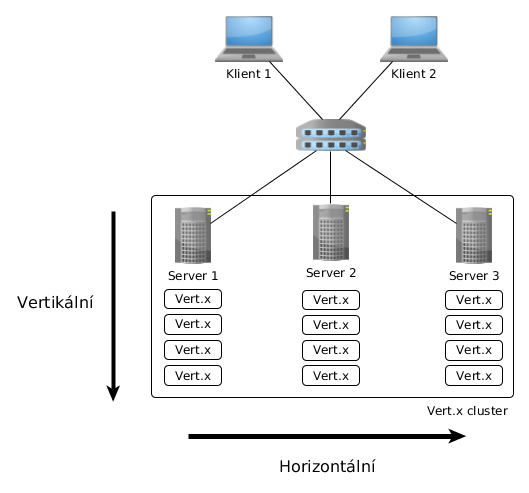
\includegraphics[scale=0.5]{obrazky/scaling_example}
\par\end{centering}
\caption{Horizontální a vertikální škálování\label{fig:scaling_example}}
\end{figure}

Díky integraci Hazelcastu získala platforma Vert.x řadu zajímavých vlastností, mezi které patří také možnost horizontálního škálování. Jak je vidět z obrázku \ref{fig:scaling_example}, jde o typ škálování do šířky propojováním více serverových instancí dohromady. Na těchto instancích běží Vert.x platforma respektive Hazelcast, který spojuje všechny klienty dohromady. To v praxi znamená, že můžeme aplikace jednoduše škálovat přes více serverů bez nutnosti běhu dalších služeb a režijních nákladů. Přímo za běhu aplikace lze přidávat další Vert.x instance do clusterů. Samotná konfigurace clusteru není nic složitého a odehrává se v souboru \emph{conf/cluster.xml} a spočívá v nastavení členů clusteru nebo specifikování multicastové\footnote{logický identifikátor skupiny sítových hostů} adresy a portu, na které bude Hazelcast po startu vyhledávat členy clusteru. Pro spuštění aplikace v režimu cluster ji stačí spustit s parametrem \emph{-cluster}. Pokud se na daném serveru nachází více síťových rozhraní je potřeba specifikovat \emph{-cluster-host}. Na tomto rozhraní bude komunikovat Hazelcast. V kapitole \ref{sub:praktCluster} je tato možnost využita pro běh Vert.x clusteru na odlišném rozhraní než běží webový server.
Velkou nevýhodou je nemožnost nasadit cluster na veřejné síti. V současné době Event Bus nepodporuje šifrované zprávy a jediná možnost, jak toho dosáhnout, je pomocí nejrůznějších privátních tunelů. Ve verzi 3.0 má být plně implementována šifrovaná komunikace a nebude již nic bránit nasazení na veřejné síti.
%Velkou výhodou je pak možnost šifrované komunikace, díky čemuž odpadá nutnost použití nejrůznějších služeb zajištující šifrování komunikace na sítové vrstvě v případě nasazení na veřejné síti nebo ve více geografických lokacích. 

\begin{figure}
\begin{centering}
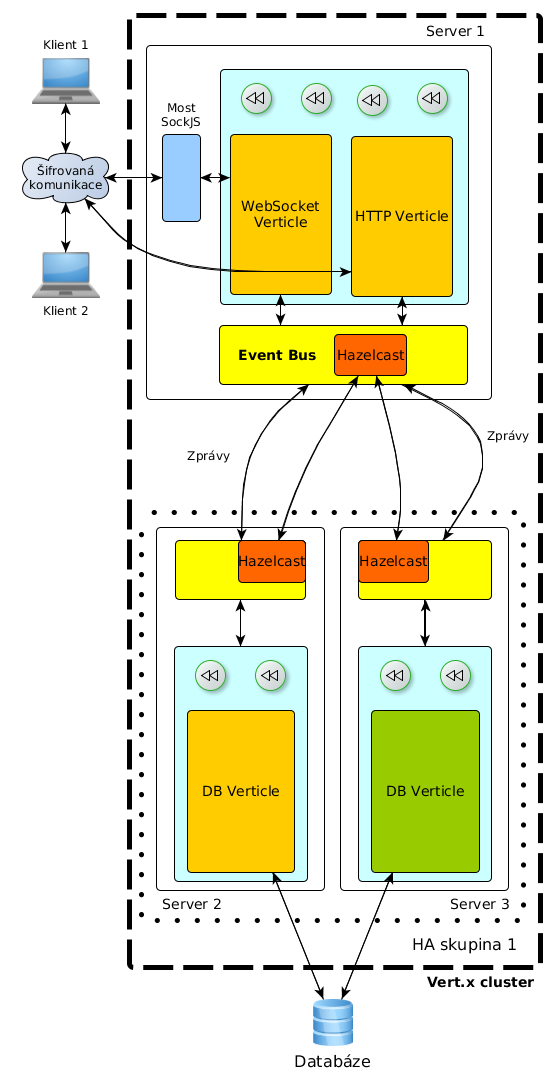
\includegraphics[scale=0.5]{obrazky/instance4_eventbus_geolocation}
\par\end{centering}
\caption{Clustering mezi třemi Vert.x instancemi \label{fig:instance4_eventbus_geolocation}}
\end{figure}

\subsection{Vysoká dostupnost}

Samostatnou kapitolou v oblasti clusteringu je HA\footnote{HA - High Availability} česky tedy vysoká dostupnost. Díky Hazelcastu ji lze řešit již na aplikační úrovni, a není potřeba  dalších služeb, které řeší vysokou dostupnost.

\subsubsection{Automatické zotavení z havárie}

Pokud je modul spuštěn s argumentem \emph{-ha} a dojde k pádu Vert.x instance. Modul bude automaticky nasazen na jiné instanci v clusteru. V takovém případě již není potřeba spouštět modul s parametrem \emph{-cluster}. Jak je vidět na obrázku \ref{fig:instance4_eventbus_geolocation}, v případě pádu Serveru 2 tedy části aplikace, která komunikuje s databází dojde automaticky k novému nasazení této části do nové instance, která je taky členem Vert.x clusteru. Výpadek tak bude pro uživatele skoro nepostřehnutelný.

\subsubsection{HA skupiny}

V případě spuštění modulů v režimu HA lze specifikovat logické skupiny. Pro spuštění instance v určité HA skupině stačí přidat parametr \emph{-hagroup <jméno skupiny>}. Díky tomu lze přesně určit, kde se mají moduly v případě pádu nasadit. To je v praxi vhodné především v situacích, kdy je do internetu vystavena pouze část clusteru. Například jako na obrázku \ref{fig:architecture_ideal}.

\subsubsection{Kvorum}

Při spuštění Vert.x instance lze specifikovat kvorum\footnote{minimální počet serverů pro zajištění vysoké dostupnosti}. Pokud nebude splněno kvorum, nebude instance nasazena v režimu HA. Kvorum lze snadno spočítat ze vzorce \\ \emph{Q = 1 + N/2}, kde N je počet serverů. Pokud dojde při běhu aplikace k porušení kvora bude režim HA automaticky vysazen.

\subsection{Vertigo cluster}

Důkazem jak dobrá je architektura, je rozšíření samotné funkcionality clusteru. Modul Vertigo\cite{vertigo}, obohacuje platformu o značné možnosti v oblasti clusterování. Jak píše sám autor projektu \emph{,,Vertigo kombinuje koncept real-time systémů a Flow-based programování."}. Architektura Vertigo by vydala sama na celou bakalářskou práci. Proto jen ve stručnosti. Vertigo podporuje dávkování zpráv mezi komponentami. Umožňuje vytváření a monitorování sítí mezi clustery a podporuje živou změnu bez restartu těchto sítí. Usnadňuje distribuci modulů přes celý cluster pro snadné nasazení v kterémkoliv jeho koutě z kteréhokoliv jeho místa.

\section{Porovnání s Node.js}

V následující kapitole bude porovnána platforma Vert.x s již zmíněnou platformou Node.js. Výkonnostní test\cite{benchmarkTim} je převzat od samotného autora projektu a jsou v něm zahrnuty jazyky, které v té době platforma podporovala. V druhé části kapitoly \ref{sub:performence} je tabulka \ref{table:odezvy}, srovnání odezev s vybranými webovými platformami s daty ze zdroje\cite{benchmark}.

\subsection{Výkon}\label{sub:performence}

Tato kapitola se zabývá výkonnostními testy jednotlivých platforem. V prvním testu je obsaženo více programovacích jazyků, ve kterých byla implementována stejná logika pod platformou Vert.x. Rychlost aplikace implementované v jiném jazyce než Javě je závislá na konkrétním adaptéru.

\subsubsection{Metody testování}

V obou testech je testovaná aplikace škálovaná na šest procesorových jader, tedy byla spuštěna s parametrem \emph{-instances 6}, oproti tomu je spuštěna aplikace Node.js ve dvou variantách. Samostatná a šest procesů v jednom clusteru. V legendě grafů je to odlišeno příponou \emph{cl}.

\begin{enumerate}
\item{Triviální dotazování serveru a návrat statusu 200\footnote{HTTP status - OK}}
\item{Dotaz na statický soubor o velikosti 72 bytů}
\end{enumerate}

\subsubsection{Hardware}

V prvním testu od Tima Foxe je požit  AMD Phenom II X6, 8GB RAM a systém Ubuntu 11.04. Tento procesor se 6 jádry není úplně běžný, proto je výklad doplněn o druhý test, který proběhl na Sandy Bridge Core i7-2600K, 8GB RAM a SSD disku a systému Ubuntu 12.04.

\subsubsection{Výsledky}

Jak lze vidět na obrázku \ref{fig:test1} a \ref{fig:test2} výsledky obou testů lze shrnout do jedné věty. Vert.x zvládá řádově o desítky tisíc více odpovědí než platforma Node.js, a to i v případě režimu clusteru.

\begin{figure}[h]
\begin{centering}
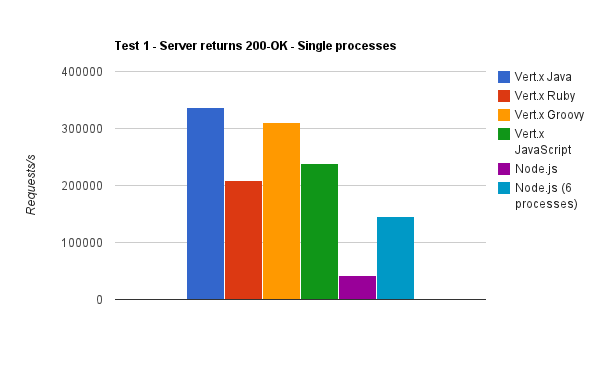
\includegraphics[scale=0.7]{obrazky/chart_1}
\par\end{centering}
\caption{Výsledky prvního testu \emph{Tim Fox} \cite{benchmarkTim}\label{fig:test1}}
\end{figure}

\begin{figure}[h]
\begin{centering}
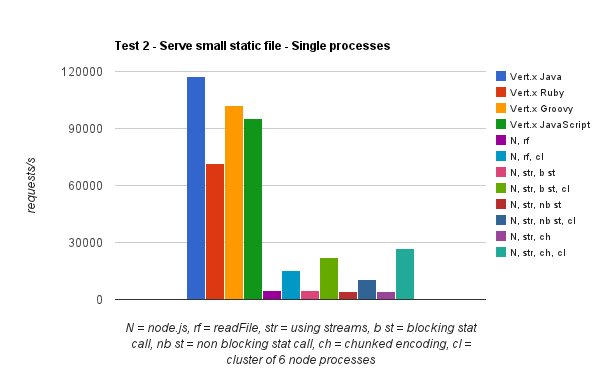
\includegraphics[scale=0.7]{obrazky/chart_3-5}
\par\end{centering}
\caption{Výsledek druhého testu \emph{Tim Fox} \cite{benchmarkTim}\label{fig:test2}}
\end{figure}

\newpage

\subsubsection{Srovnání s vybranými platformami}

Metoda srovnání s ostatními platformami je založená na podobném principu jako předchozí testy, s tím rozdílem, že místo statického souboru vrací odpověď ve formátu JSON. Na straně serveru tedy musí dojít k JSON serializaci.

\begin{table}[h]
\centering
\caption{Srovnání odezvy, \emph{převzato a upraveno z} \cite{benchmark}}
\begin{tabular}{ |c|c|c| }
\hline
\textsf{\textbf{Platforma}} & \textsf{\textbf{Průměrná odezva}} & \textsf{\textbf{Maximální}}\tabularnewline
\hline
Vert.x & 1,2ms & 18,7ms\tabularnewline
\hline 
Netty & 1,3ms & 24,0ms\tabularnewline
\hline
Ruby on Rails & 1.8ms & 241.6\tabularnewline
\hline 
Node.js & 3.7ms & 12,5\tabularnewline
\hline
\end{tabular}
\label{table:odezvy}
\end{table}

\newpage

\subsection{Vlastnosti}

Následující tabulka ukazuje srovnání důležitých vlastností jednotlivých platforem, jejichž důležitost byla popsána v předchozích kapitolách.
\begin{table}[h]
\centering
\caption{Srovnání vlastností s Node.js}
\begin{tabular}{ |c|c|c| }
\hline
\textsf{\textbf{Vlastnost}} & \textsf{\textbf{Node.js}} & \textsf{\textbf{Vert.x}}\tabularnewline
\hline
CLI & Ano & Ano\tabularnewline
\hline 
Cluster & Ano & Ano\tabularnewline
\hline
Moduly & Ano & Ano\tabularnewline
\hline 
HA & Ne & Ano\tabularnewline
\hline
MQ & Ne & Ano\tabularnewline
\hline 
Hybridní model vláken & Ne & Ano\tabularnewline
\hline 
In-memory data grid & Ne & Ano\tabularnewline
\hline 
Polyglot & Ne & Ano\tabularnewline
\hline
\end{tabular}
\end{table}

\subsection{Závěr srovnání}

Výsledkem srovnání je tedy fakt, že pokud by se dnes někdo rozhodoval o výběru platformy pro novou real-time aplikaci, měl by určitě zvolit platformu Vert.x, která poskytuje větší výkon a počet vlastností, nehledě na fakt, že v případě Node.js lze psát aplikaci pouze v jazyce JavaScipt, který se může jevit jako naprosto nevhodný pro Enteprise aplikaci.

\section{Budoucnost projektu}

Tim Fox hlavní vedoucí projektu představil plán\cite{plan} pro budoucí rozvoj platformy. Nově tak bude šifrovaná veškerá komunikace na Event busu. API bude definováno pomocí vysoce abstraktního programovacího jazyka díky čemuž bude možné generovat API v jiných programovacích jazycích. Zveřejnění jednoduchého protokolu pro napojení na Event Bus což de v současné době pouze přes WebSocket a SockJS most. Objevit by se měla také nativní podpora pro Android a IoS. Je dobře, že vývoj jde stále dopředu a umožňuje tím rozšířit okruh programátorů.